\chapter{Conclusions}\label{cha:conclusion}
\epigraph{`Difficulties mastered are opportunities won.'}{\mbox{\textup{\textsc{Winston Churchill}}}}
%
This work has tested two silicon cold-electron bolometers and assessed their potential, predominately in terms of their sensitivity. The two detectors tested were fabricated to the same designs, differing only in the material used to construct the detector's absorber. The first detector tested used an unstrained \textit{control} silicon material, which was heavily doped (with phosphorus to a concentration of $4\times 10^{19}~\mathrm{cm^{-3}}$); whereas, in the second device, the absorbing silicon was strained (through a \ce{Si_{0.7}Ge_{0.3}} layer), as well as being doped to the same concentration as in the previous detector (the cross-sections of the two wafers used are shown in Figures~\ref{fig:CEB_crossSection} and \ref{fig:CEB_crossSection_strained}, respectively). For both detectors, radiation was coupled to the absorber via a twin-slot antennae, designed to couple radiation with a frequency of $160~\mathrm{GHz}$ (the antenna design has been detailed in Section~\ref{ssec:antenna}).
\par 
Both detectors have been measured in the absence of optical power (dark measurements, Chapter~\ref{cha:darkResults}) and with incident optical power from black-body sources (Chapter~\ref{cha:opticalResults}). Dark measurements predominately consisted of measuring the current-voltage relationship of the detectors as the phonon (bath) temperature was varied. The results of these measurements (shown in Figures~\ref{fig:controlIVs} and \ref{fig:strainedIVs} for the unstrained and strained devices, respectively) verified that tunnelling junctions had been formed between the silicon absorber and the superconducting (aluminium) contacts. These data also allowed the electron-cooling performance to be calculated (by fitting to Equation~\ref{res:IV}); by doing so, the ability of these detectors to cool the carriers in the silicon absorber to below the temperature of the lattice has been demonstrated (see Figures~\ref{fig:controlTe} and \ref{fig:strainedTe}). The electron-temperature fitting showed the benefits of using strained silicon, in that the strained-silicon detector was able to cool the electrons in the silicon to a lower temperature than the unstrained device (the strained detector was able to cool electrons to $\approx 100~\mathrm{mK}$ compared to $\approx 180~\mathrm{mK}$ for the unstrained silicon; in both cases, the bath temperature was $300~\mathrm{mK}$); this improved performance is the result of the reduced coupling between the electrons and phonons in the strained material.
\par 
These tests were repeated with the detectors illuminated by a black-body source. From these measurements, it was clear that a response to a change in optical power (produced by varying the temperature of the black-body source) could be measured in the \gls{acr:IV} curves and thus, it would be possible to measure a varying optical signal by biasing the device at a constant value (Figures~\ref{fig:controlIVs_optical} and \ref{fig:strainedIVs_optical} show the current-voltage relationship for the unstrained and strained detectors, respectively, for different levels of optical power). By using the same electron-temperature fitting technique used for the dark data, along with Equation~\ref{eqn:Pabs_V0} (the absorbed power) and Equation~\ref{res:Iresponsivity} (the responsivity in a current-biased regime), the responsivity was calculated to peak at $2.1 \times 10^{6}~\mathrm{V\,W^{-1}}$ for the unstrained detector and $1.5 \times 10^{7}~\mathrm{V\,W^{-1}}$ for the strained-silicon detector (these results are taken from Figures~\ref{fig:controlResponsivity} and \ref{fig:strainedResponsivity}, respectively). This factor of $10$ is approaching, but noticeably less than, the difference in the electron-phonon coupling which was $29$ (from Table~\ref{tab:materialProperties}). This still represents a strong advantage in the performance of the strained detector compared to the unstrained device. This improvement is the result of the weaker electron-phonon coupling (as discussed in Section~\ref{sec:eph}) present in the strained detector, which allows the electrons to heat up by a greater amount per unit amount of optical power incident; this is seen by comparing the temperatures of the carriers at zero bias in the case of each detector (see Figures~\ref{fig:controlTe_optical} and \ref{fig:strainedTe_optical}). There should be no significant difference in the sensitivity of the tunnelling-junction thermometers between the two cases.
\par 
As well measuring the current-voltage behavior of the detector under optical loading, the electrical noise was also measured as a function of optical load and bias. These data, combined with those already collected and the various equations presented in Section~\ref{sec:theory-NEP}, allowed for a complete model of the noise-equivalent power of each detector to be produced (these have been presented in Figure~\ref{fig:controlNoiseModel77} for the unstrained detector and Figures~\ref{fig:strainedNoiseModel300} and \ref{fig:strainedNoiseModel77} for the strained-silicon detector). The results of these measurements are summarised for comparison in Figure~\ref{fig:NEPcomparison}. This graph compares the device-limited noise of the two detectors; it is clear that the inherent noise of the strained-silicon detector is lower than that of the unstrained device (by a factor of approximately 3.5). In both cases, the device noise was limited by the flow of charges through the tunnelling contacts, a combination of the final three terms in Equation~\ref{res:NEP_CEB}. When other noise sources such as the readout amplifier and photon noise---which were the limiting sources for the unstrained and strained detectors, respectively---are considered, the achieved noise-equivalent powers were $1.5 \times 10^{-16}~\mathrm{W\,Hz^{\nicefrac{-1}{2}}}$ and $6.6 \times 10^{-17}~\mathrm{W\,Hz^{\nicefrac{-1}{2}}}$ for the unstrained and strained detectors, respectively. From this, and when considering both the extremely early stage of development and the unoptimised designs used here, it has been shown that silicon cold-electron bolometers have the potential to rival the most sensitive detectors operating in the far infrared \parencite[such as those reported by:][]{Suzuki2014,deVisser2014,Karasik2015}.
\begin{figure}[tb]
\begin{center}
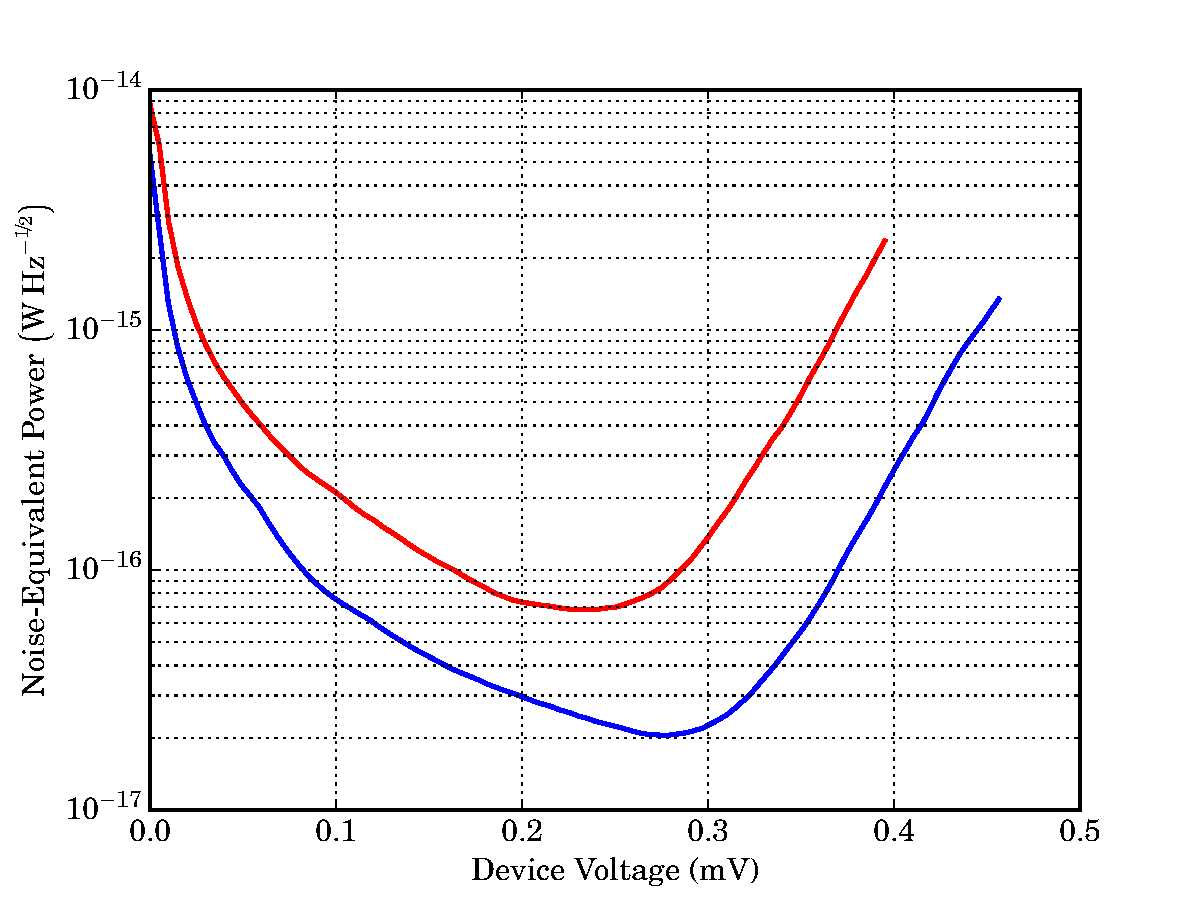
\includegraphics[width = 0.95\textwidth]{figures/NEP_comparison}
\caption[Comparison between device-limited noise-equivalent power for silicon cold-electron bolometers made with unstrained and strained silicon]{Comparison between device-limited noise-equivalent power for silicon cold-electron bolometers made with unstrained (red) and strained (blue) silicon, at a thermal bath temperature of $350~\mathrm{mK}$.}
\label{fig:NEPcomparison}
\end{center}
\end{figure}
\par 
Attempts were made to determine the time constant of the strained-silicon detector by measuring the response to a rapidly-chopped source and by measuring the roll-off in photon noise. Neither of these methods were able to accurately determine the time constant, instead only upper limits could be inferred; these were $\tau < 14~\mathrm{\upmu s}$ from the chopped optical source and $\tau < 1.5~\mathrm{\upmu s}$ from the roll-off in photon noise. These values not only match or better the current state-of-the-art detectors operating in these wavelengths \parencite[e.g.][]{Zhang2015,deVisser2014,Karasik2011} but also show that such detectors are indeed capable of achieving the anticipated time constant of $10~\mathrm{ns}$ presented by \textcite{Kuzmin2004}.
\par 
These results \parencite[which have been, in part, previously published in][]{Brien2014} represent the first optical measurements for a silicon cold-electron bolometer, as well as some of the first optical result for any type of cold-electron bolometer. To put the results presented in this thesis in the context of the wider field, Table~\ref{tab:compCEBs} compares the results obtained for the two devices studied here with those achieved in recent years for metal-based cold-electron bolometers. It can be seen that, considering the early stage of development, the strained-silicon cold electron bolometer compares well.
\begin{table}[htb]
\caption[Comparison of the optical performance of various cold-electron bolometer reported in recent years]{Comparison of the optical performance of various cold-electron bolometer reported in recent years.} 
\label{tab:compCEBs}
\centering
\begin{threeparttable}
\begin{tabular}{llll}
\toprule\toprule
Detector & \parbox{\widthof{Absorber Volume}}{Absorber Volume \\$\left(\mathrm{m^{3}}\right)$}& \parbox{\widthof{Power $\left(\mathrm{W\,Hz^{\nicefrac{-1}{2}}}\right)$}}{Noise-Equivalent\\Power $\left(\mathrm{W\,Hz^{\nicefrac{-1}{2}}}\right)$} 
& \parbox{\widthof{Responsivity}}{Responsivity\\$\left(\mathrm{V\,W^{-1}}\right)$} \\
\midrule
Unstrained SiCEB & $1.3 \times 10^{-17}$ & $2.4 \times 10^{-16}$ & $2.7 \times 10^{6}$\\
Strained SiCEB & $1.3 \times 10^{-17}$ & $6.6 \times 10^{-17}$ & $1.5 \times 10^{7}$\\
\parbox{\widthof{Aluminium CEBa}}{Distributed\\Aluminium CEB\tnote{a}} & $8 \times 10^{-20}$ & $4.8 \times 10^{-17}$ & $8.8 \times 10^{8}$\\
Titanium CEB\tnote{b} & \textit{Not given} & $8.9 \times 10^{-17}$ & $1.1 \times 10^{8}$\\
\bottomrule
\end{tabular}
\begin{tablenotes}
\item[a] \textcite{Tarasov2011}.
\item[b] \textcite{Otto2013}.
\end{tablenotes}
\end{threeparttable}
\end{table}
\par 
As discussed in Chapter~\ref{cha:introduction}, it is a goal for the next generation of space-based instruments to operate at noise-equivalent powers of close to $10^{-20}~\mathrm{W\,Hz^{\nicefrac{-1}{2}}}$. While promising for a prototype device, the results presented here, along with those shown in Table~\ref{tab:compCEBs}, are still orders of magnitude above this. In the absence of noise due to either photons or readout, the limiting noise performance of a silicon cold-electron bolometer is due to the tunnelling noise (Equations~\ref{eqn:NEP_P}, \ref{eqn:NEP_shot} and \ref{eqn:NEP_PI}) and the noise due to the electron-phonon interactions (Equation~\ref{eqn:NEP_e-ph}). In order to ascertain if the technology presented here could achieve a \gls{acr:NEP} of approaching $10^{-20}~\mathrm{W\,Hz^{\nicefrac{-1}{2}}}$, a similar noise model to those presented in Chapter~\ref{cha:opticalResults}, but with the dimensions of the detector reduced by a factor of a hundred and the operating temperature reduced by a factor of three, has been performed. This model gives a very approximate limit of $1\mbox{--}2 \times 10^{-18}~\mathrm{W\,Hz^{\nicefrac{-1}{2}}}$ for such a device. This is limited by the tunnelling noise; the noise due to the electron-phonon noise-equivalent power in such a detector is estimated to be approximately $6 \times 10^{-20}~\mathrm{W\,Hz^{\nicefrac{-1}{2}}}$. This shows some promise for such detectors, however improvements are needed to bring the overall noise-equivalent power down to the level of $10^{-20}~\mathrm{W\,Hz^{\nicefrac{-1}{2}}}$. The current noise contribution to the tunnelling noise reduces with the responsivity (which has not been altered in this model) as $S^{-1}$, as seen in Equation~\ref{eqn:NEP_shot}. As such, improving the responsivity should bring the over noise-equivalent power down. As discussed in Section~\ref{sec:opticalStrainedSi}, the presence of strain in the absorber has the effect of increasing the responsivity of a silicon cold-electron bolometer, as the electrons are heated more per unit of power absorbed. As discussed in Section~\ref{sec:eph}, the thermal conduction between electrons and phonons in the strained material is currently much higher than models would suggest and, as such, improvements to the straining of the absorber are definitely plausible and should help to improve the overall noise-equivalent power of these detectors.
\par
To perform the measurements described in this work, a bias and readout system has been designed and revised for best performance. To facilitate the  measurement of the very low noise voltage associated with these detectors, a novel means of measuring below the amplifier noise floor has been described. This was performed by cross correlating the output of two matched amplifiers to remove the uncorrelated amplifier noise. This technique has been shown to reduced the noise associated with the readout chain from $\approx 1~\mathrm{nV\,Hz^{\nicefrac{-1}{2}}}$ to $300~\mathrm{pV\,Hz^{\nicefrac{-1}{2}}}$ with averaging (shown in Figure~\ref{fig:crossCol_NoiseSimData}). This technique clearly has great potential for measuring ultra-low noise sources to determine the characteristics of high-end devices.
\par 
In order to explain the spectral responses seen in Figures~\ref{fig:controlSpectrum} and \ref{fig:strainedSpectrum}, the simulation work of the optical system has been revisited in much greater detail than was initially performed. This work showed that the main source degradation in the spectral response was the silicon lens, which was lacking any anti-reflection coatings. It also showed that the DC cuts in the ground plane (which were essential for biasing the detector) had added to the spectral response at frequencies other than the design frequency.
\par 
A brief study has been performed to determine if the silicon material used to fabricate these detectors may place a limit on the usable frequency range of detectors fabricated using it. This work (presented in Section~\ref{sec:siliconFTS}) showed that while no severe limit exists, both materials exhibited small drops in absorption beyond a few THz. This drop should not by any means make the construction of a silicon cold-electron bolometer operating above this frequency implausible.
\par 
This work has only performed an initial study of silicon cold-electron bolometers. Clearly, there is a great scope for further study and refinement of these detectors, to deduce those properties that have not been accurately found in this work and to work towards improving those which already have. It is the opinion of the author that the logical next step in this work is to accurately measure the time constant of such a detector. Based on the findings of this work, the best route to achieve this would be to measure the photon noise to higher readout frequencies than those studied here and to measure the roll-off in this noise.
\par 
This work has only studied the behavior of detectors under a very limited set of optical loadings, there should be great interest in a more complete study, from which the dynamic range of these detectors could be ascertained along with constraining, through measurement, the relationship between the responsivity and the absorbed optical power. Beyond this, a more optimised device could be fabricated and tested to compare with the detectors studied in this work. Such detectors should have smaller overall dimensions (reducing the electron-phonon noise), along with more controlled---higher-quality---tunnelling contacts. It is envisaged that such a device should be capable of offering at least an order of magnitude improvement to the sensitivity (if not more), with no tradeoff to other characteristics. In fact, such a device may well improve on the time constant of the designs presented in this work, since their relatively large absorber size may result in the time constant being limited by the diffusion time of the electrons in the absorber, rather than the tunnelling time.
\par 
Overall, this thesis has, through thorough testing of two types of silicon cold-electron bolometer, demonstrated that such devices are highly sensitive detectors capable of operating with very short time constants. Furthermore, it has been shown that this is possible even for a proof-of-concept type detector lacking optimisation. With relatively simple refinements to both design and the fabrication, these detectors clearly present a very exciting opportunity to achieve the ultra-low noise limits which will be required by the next generation of space-based far-infrared observatories.

 
